\documentclass[twocolumn, 8pt]{extarticle}

% Uncomment to squeeze everything onto one side
\usepackage{pgfpages}
\pgfpagesuselayout{2 on 1}[letterpaper, landscape]

\usepackage[letterpaper,margin=0.25in]{geometry}
\input{ncommon}
\everymath{}
\usepackage{titlesec}
\usepackage{multicol}

\usepackage[english]{babel}
\usepackage[autostyle]{csquotes}
\MakeOuterQuote{"}

% Options: [subtle], [moderate], or [extreme]
\usepackage[extreme, mathspacing=normal, lists=normal]{savetrees} 
% Restore space between operators (sin, cos, log) and variables
% \thinmuskip=3mu       % Readable sin/cos
% \medmuskip=2mu        % Tight + and -
% \thickmuskip=3mu      % Tight =
\usepackage{enumitem}

\newenvironment{tight}
  {\begingroup
   \setlength{\arraycolsep}{2pt}
   \thinmuskip=3mu       % Readable sin/cos
   \medmuskip=2mu        % Tight + and -
   \thickmuskip=3mu      % Tight =
  }
  {
    \endgroup
  }


% Normal vdots and ddots leave too much space above
% https://tex.stackexchange.com/questions/207056/wrong-too-much-vertical-space-above-vdots-in-small-matrix
\newcommand{\newvdots}{\vphantom{\int\limits^x}\smash[t]{\vdots}}
\newcommand{\newddots}{\vphantom{\int\limits^x}\smash[t]{\ddots}}

\titleformat{\section}
  {\normalfont\fontsize{12}{14}\bfseries}{\thesection}{1em}{}
\titlespacing\section{0pt}{5pt plus 2pt minus 2pt}{2pt plus 1pt minus 1pt}
\titlespacing\subsection{0pt}{5pt plus 2pt minus 2pt}{2pt plus 1pt minus 1pt}
\titlespacing\subsubsection{0pt}{5pt plus 2pt minus 2pt}{2pt plus 1pt minus 1pt}
%\renewcommand{\arraystretch}{1.5}
\setlist{nosep}
\setlength{\abovedisplayskip}{3pt}
\setlength{\belowdisplayskip}{3pt}
\setlength{\abovedisplayshortskip}{0pt}
\setlength{\belowdisplayshortskip}{3pt}
\setlength{\parindent}{0pt}
\setlength{\parskip}{2pt}
\raggedbottom
\raggedcolumns

\title{ROB521 Exam Aidsheet}
\author{Tyler Tian}

\begin{document}

\section{Mathematical Foundations} %%%%%%%%%%%%%%%%%%%%%%%%%%%%%%%%%%%%%%%%%%%%%%%%

\textbf{Skew-Symmetric Operator:}
\begin{gather*}
\bm r^\times = \matthree[bsmall]{0}{-r_3}{r_2}{r_3}{0}{-r_1}{-r_2}{r_1}{0} \quad \bm x^T\bm w^\times\bm x = 0 \quad
\bm C\bm w^\times\bm C^T = [\bm C\bm w]^\times, \bm C \in SO(3)
\end{gather*}

\textbf{Singularity/Constraint Dilemma:} There is no representation of rotations that has exactly 3 parameters
(i.e. no constraints) and also no singularities.

\textbf{Rotation Matrices:} \(\bm C_{21} = \vcx F_2 \cdot \vcx F_1^T \implies \bm r_2 = \bm C_{21}\bm r_1\).
\(\bm C^T\bm C = \bm 1, \det\bm C = 1\).

\textbf{Principal Rotations:} Transforms between this frame and a frame obtained by rotating about an axis by an
angle. \emph{Note the notation here is the opposite of what's used in most other courses. The matrices used to rotate a
vector about a coordinate axis are the inverse of the matrices here.}
\[
\bm C_1(\theta) = \matthree[bsmall]{1}{0}{0}{0}{\cos\theta}{\sin\theta}{0}{-\sin\theta}{\cos\theta} \quad
\bm C_2(\theta) = \matthree[bsmall]{\cos\theta}{0}{-\sin\theta}{0}{1}{0}{\sin\theta}{0}{\cos\theta} \quad
\bm C_3(\theta) = \matthree[bsmall]{\cos\theta}{\sin\theta}{0}{-\sin\theta}{\cos\theta}{0}{0}{0}{1}
\]
\textbf{Euler Angles:} One of 12 compositions of principal rotations. Has singularities.

\textbf{Axis-Angle:} \(\bm C = \cos(\phi)\bm 1 + (1 - \cos\phi)\bm a\bm a^T - \sin\phi\bm a^\times\) constraint \(\bm a^T\bm a = 1\).

\textbf{Quaternion:} \(\bm q = q_0 + \brm q = q_0 + q_1i + q_2j + q_3k \in \mathbb H\) are normalized to be unit length on \(\mathbb S^3\),
which forms a \textbf{double cover} of \(SO(3)\).
\(\bm q\) is the same rotation as \(-\bm q\). \(\bar{\bm q}\) (conjugate) is the opposite rotation.
% Multiply as \[\bm p \otimes \bm q = (p_0 + \bm{\mathrm p}) \otimes (q_0 + \bm{\mathrm q}) = p_0q_0 - \bm{\mathrm p}^T\bm{\mathrm q} + p_0\bm{\mathrm q} + q_0\bm{\mathrm p} + \bm{\mathrm p} \times \bm{\mathrm q}\]
\(\bm q = \cvec{\eta}{\bm\varepsilon} = \cvec{\cos(\phi/2)}{\bm a\sin(\phi/2)}\).
\(\bm C = (\eta^2 - \bm\varepsilon^T\bm\varepsilon)\bm 1 + 2\bm\varepsilon\bm\varepsilon^T - 2\eta\bm \varepsilon^\times\).

\textbf{Gibbs Vector:} \(\bm C = (1 + \bm g^\times)^{-1}(1 - \bm g^\times), \bm g = \bm a\tan\frac{\phi}{2}\)

\textbf{Infinitesimal Rotations:} \(\bm C = 1 - \bm\theta^\times\) where \(\bm\theta = \phi\bm a\).

\textbf{Velocity in Another Frame:} \(\uvec r^\dota = \uvec r^\dotb + \uvec\omega _{21} \times \uvec r \iff
\dot{\bm r}_1 = \bm C_{12}(\dot{\bm r}_2 + {\bm\omega _2^{21}}^\times\bm r_2)\)

\textbf{Poisson's Equation:} \(\dot{\bm C}_{21} = -{\bm\omega _2^{21}}^\times\bm C_{21}\)

\textbf{Transforms:} \(\bm r_i^{pi} = \bm C_{iv}\bm r_v^{pv} + \bm r_i^{vi} \Leftrightarrow \cvec{\bm r_i^{pi}}{1} = \mattwo{\bm C_{iv}}{\bm r_i^{vi}}{\bm 0^T}{1}\cvec{\bm r_v^{pv}}{1} = \bm T_{iv}\cvec{\bm r_v^{pv}}{1}\)

Note vehicle pose is \(\bm T_{iv}\) (vehicle-to-inertial), not \(\bm T_{vi}\)!

\textbf{Inversion:} \(\bm T_{iv}^{-1} = \mattwo{\bm C_{iv}^T}{-\bm C_{iv}^T\bm r_i^{vi}}{\bm 0^T}{1} = \mattwo{\bm C_{vi}}{-\bm r_v^{vi}}{\bm 0^T}{1} = \mattwo{\bm C_{vi}}{\bm r_v^{iv}}{\bm 0^T}{1} = \bm T_{vi}\)

\textbf{Combined Velocity:} \(\bm\varpi _v^{vi} = \cvec{\bm\nu ^{vi}}{\bm\omega _v^{vi}}, \dot{\bm T}_{vi} = \mattwo{{\bm\omega _v^{vi}}^\times}{-\bm\nu _v^{vi}}{\bm 0^T}{0}\bm T_{vi}\)

\section{Vehicle Modelling} %%%%%%%%%%%%%%%%%%%%%%%%%%%%%%%%%%%%%%%%%%%%%%%%

\subsection{Wheel Kinematics}

\begin{center}
  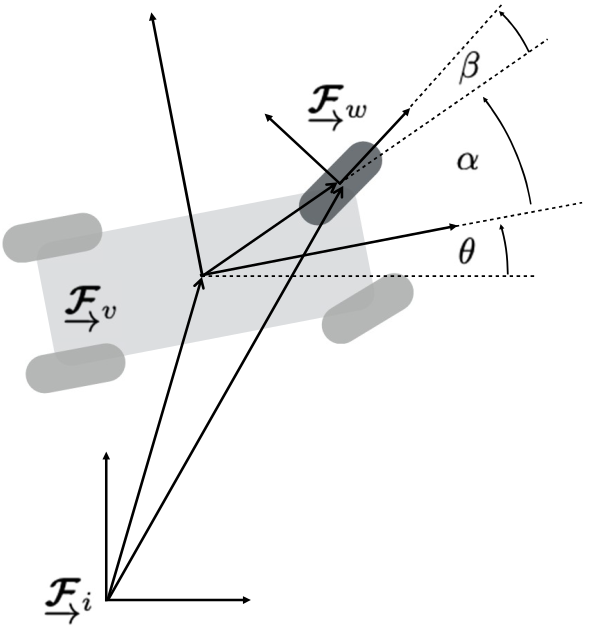
\includegraphics[width=0.3\linewidth]{imgs/diffkine.png}
  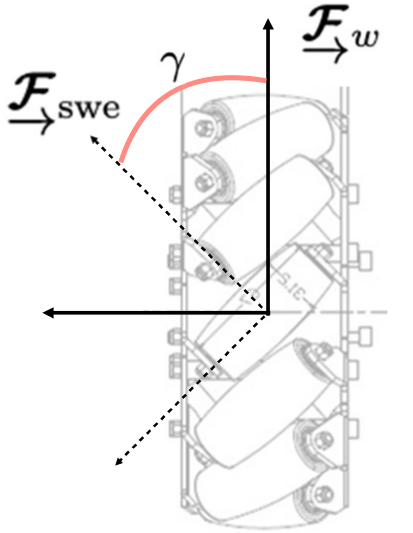
\includegraphics[width=0.2\linewidth]{imgs/swedish.png}
\end{center}

For a standard wheel with radius \(r\), rotation \(\varphi\):
\begin{align*}
  \rvec{\cos(\alpha + \beta)}{\sin(\alpha + \beta)}{d\sin\beta}\dot{\bm\xi} &= \dot\varphi r \\
  \rvec{-\sin(\alpha + \beta)}{\cos(\alpha + \beta)}{d\cos\beta}\dot{\bm\xi} &= 0
\end{align*}
where \(\dot{\bm\xi} = \rvec{v}{u}{\omega}^T\) is the vehicle-frame pose rate.
Solving for \(\dot\varphi\) yields \textbf{inverse differential kinematics}.
Solving for \(\dot{\bm\xi}\) (by pseudoinverse \((\bm A^T\bm A)^{-1}\bm A^T\)) yields \textbf{forward differential kinematics}.

For Swedish wheels with rollers at angle \(\gamma\) (\(\dot\varphi _s\) usually unconstrained):
\begin{align*}
  \rvec{\cos(\alpha + \beta + \gamma)}{\sin(\alpha + \beta + \gamma)}{d\sin(\beta + \gamma)}\dot{\bm\xi} &= \dot\varphi r\cos\gamma + \dot\varphi _sr_s \\
	\rvec{-\sin(\alpha + \beta + \gamma)}{\cos(\alpha + \beta + \gamma)}{d\cos(\beta + \gamma)}\dot{\bm \xi} &= -\dot\varphi r\sin\gamma
\end{align*}

\textbf{Differential Drive Kinematics:} Origin halfway between wheels (\(b\) from wheels).
\[
\cvec{\dot\varphi _r}{\dot\varphi _l} = \frac{1}{r}\mattwo{1}{b}{1}{-b}\cvec{v}{\omega} \qquad \cvec{v}{\omega} = \frac{1}{2}\mattwo{r}{r}{r/b}{-r/b}\cvec{\dot\varphi _r}{\dot\varphi _l}
\]

\subsection{Euler-Lagrange}

Nonholonomic constraints written as \(\bm H(\bm q)^T\dot{\bm q} = \bm 0\) where \(\bm q = \rvec{x}{y}{\theta}^T\).
Null space of \(\bm H(\bm q)^T\) are admissible velocities \(\dot{\bm q} = \bm G(\bm q)\bm p\) where \(\bm p\) is
generalized velocity and \(\bm H(\bm q)^T\bm G(\bm q) = \bm 0\).

\textbf{Euler-Lagrange Equation:} \(\displaystyle \diff{}{t}\left(\pdiff{^TL}{\dot{\bm q}}\right) - \pdiff{^TL}{\bm q} = \bm\tau + \bm H(\bm q)\bm\lambda\)
where \(L = T - V\), \(\bm\tau = \bm G(\bm q)\bm\nu\) (generalized forces), \(\bm\lambda\) are Lagrange multipliers.
To eliminate the Lagrange multiplier term, premultiply by \(\bm G(\bm q)^T\).

\subsection{Vehicle Dynamics Models}

\textbf{Generalized Vehicle Model:} \(\dot{\bm x} = \bm A(\bm x)\bm x + \bm B(\bm x)\bm u\) where \(\bm x = \rvec{\bm q}{\bm p}^T\);
with kinematics only, \(\bm A = \bm 0\).

\textbf{Unicycle Model:} \(\cvec{\dot{\bm q}}{\dot{\bm p}} = \mattwo{\bm 0}{\bm G(\bm q)}{\bm 0}{-\bm M^{-1}\bm D}\cvec{\bm q}{\bm p} + \cvec{\bm 0}{\bm M^{-1}}\bm u\)
where
\[\bm p = \cvec{v}{\omega} \quad \bm G(\bm q) = \matthreetwo{\cos\theta}{0}{\sin\theta}{0}{0}{1} \quad
\bm M = \mattwo{m}{0}{0}{I} \quad \bm u = \cvec{f}{g} \quad \bm\nu = -\bm D\bm p + \bm u\]
for some damping \(\bm D\), thrust \(f\), steering torque \(g\).

\textbf{Bicycle Model:} \(\cvec{\dot{\bm q}}{\dot{\bm p}} = \mattwo{\bm 0}{\bm G(\bm q)}{\bm 0}{-\bm M(\bm q)^{-1}\bm D(\bm q, \bm p)}\cvec{\bm q}{\bm p} + \cvec{\bm 0}{\bm M(\bm q)^{-1}}\bm u\)
where
\[\bm q = \cvec{x}{y}{\theta}{\gamma} \quad \bm p = \cvec{v}{\varsigma} \quad \bm G(\bm q) = \mat{\mrow{\cos\theta}{0}\mrow{\sin\theta}{0}\mrow{\frac{\tan\gamma}{d}}{0}\mrow{0}{1}} \quad
\bm M = \matfour{m}{0}{0}{0}{0}{m}{0}{0}{0}{0}{I + I_f}{I_f}{0}{0}{I_f}{I_f}\]
and \(\bm M(\bm q) = \bm G(\bm q)^T\bm M\bm G(\bm q), \bm D(\bm q, \bm p) = \bm G(\bm q)^T\bm M\dot{\bm G}(\bm q) + \bm D\)
for front wheel steering angle \(\gamma\), rear wheel velocity \(v\), steering speed \(\varsigma\), distance \(d\)
between wheels.

\section{Path-Tracking Control} %%%%%%%%%%%%%%%%%%%%%%%%%%%%%%%%%%%%%%%%%%%%%%%%

\textbf{Errors:} Crosstrack error \(\varepsilon _L = y_d - y\) (distance between vehicle and closest point on path) and
heading error \(\varepsilon _H = \theta _d - \theta\) (based on path tangent at closest point).

\textbf{Feedback Linearization:} Given a nonlinear system \(\dot x = f(x) + g(x)u\), define new input \(\eta\) and find
input mapping \(u = a(x) + b(x)\eta\) such that \(\dot x = f(x) + g(x)(a(x) + b(x)\eta) = Ax + B\eta\), i.e. find \(A, B\)
such that \(f(x) + g(x)a(x) = Ax, g(x)b(x)\eta = B\eta\).

Applied to unicycle model: \(\cvec{\dot\varepsilon _L}{\dot\varepsilon _H} = \cvec{v\sin\varepsilon _H}{\omega}\)
(tangent approximation), change variables \(\cvec{z_1}{z_2} = \cvec{\varepsilon _L}{v\sin\varepsilon _H}\) to get
\(\cvec{\dot z_1}{\dot z_2} = \mattwo{0}{1}{0}{0}\cvec{z_1}{z_2} + \cvec{0}{1}\eta\) where \(\eta = v\omega\cos\varepsilon _H\).
Let output \(y = \rvec{\alpha}{1}\cvec{z_1}{z_2}\) and proportional controller \(\eta = K(y_d - y)\), take \(K = 4\alpha\)
to get \(\displaystyle \omega = -\frac{4\alpha^2}{v}\frac{\varepsilon _L}{\cos\varepsilon _H} - 4\alpha\tan\varepsilon _H\).

This has singularities at \(\varepsilon _H = \pm\pi / 2\) or \(v = 0\), and overshoots turns.

\textbf{Pure Pursuit:} Steer the robot towards a target lookahead point. Lookahead is hard to select for varying speeds;
too short results in oscillation; too long results in slow convergence.

\textbf{Stanley Controller:} For bicycle models, using front axle centre as origin,
\(\displaystyle \delta(t) = \varepsilon _H(t) + \tan^{-1}\left(\frac{k\varepsilon _L(t)}{k_s + v_f(t)}\right)\)
for some steering \(\delta(t)\) and forward velocity \(v_f(t)\), gain \(k\) and softening \(k_s\).

Error dynamics: using \(\displaystyle \dot\varepsilon _H(t) = \frac{-v_f(t)\sin(\delta(t))}{l}, \dot\varepsilon _L(t) = v_f(t)\sin(\varepsilon _H(t) - \delta(t))\),
crosstrack error has \(\displaystyle \dot\varepsilon _L(t) = \frac{-k\varepsilon _L(t)}{\sqrt{1 + \left(\frac{k\varepsilon _L(t)}{v_f}\right)^2}}\),
exponential decay for small \(\varepsilon _L\).

\textbf{Model Predictive Control:} At each step, predict all future errors for some horizon, find optimal sequence of
control inputs, apply the first step (or for a short time) and iterate again.

Parametrize control over horizon: \(\cvec{v(t)}{\omega(t)} = \cvec{v_0}{\omega _0} + \cvec{v_1}{\omega _1}t + \cvec{v_2}{\omega _2}t^2 + \cvec{v_3}{\omega _3}t^3\)
with \(v_{0..3}, \omega _{0..3}\) as parameters. Simulate with full model to minimize cost function
\(\displaystyle J(\bm u) = \frac{1}{2}\sum _i w_i\varepsilon _{L,i}^2 + \frac{1}{2}\sum _k \left(w_{v,k}v_k^2 + w_{\omega,k}\omega _k^2\right)\).

\section{Planning} %%%%%%%%%%%%%%%%%%%%%%%%%%%%%%%%%%%%%%%%%%%%%%%%

\textbf{General Approach:} A strategic/high-level (global) planner, planning an optimal route based on a priori
knowledge, and a tactical/low-level (reactive) planner that handles real-time obstacle avoidance.

\textbf{Standard Planning Sequence:} Compute a simple path, smooth the path to account for kinematics, design a
trajectory to account for dynamics (i.e. adding a velocity profile), and design a controller to track the trajectory.

\subsection{Reactive Planners}

\textbf{Potential Fields:} Define a potential \(V(x_t) = V_\text{att}(x_t) + V_\text{rep}(x_t)\) where
\(V_\text{att}(q) = K_\text{att}\rho(q, q^g)^2\) and \(\displaystyle V_\text{rep}(q) = K_\text{rep}\sum _{i = 1}^n \frac{1}{\rho(q, O^i)^2}\)
and use gradient descent (move in the direction of \(-\nabla V\)).
Can get stuck in local minima; non-optimal; does not account for vehicle constraints.

\textbf{Extended Potential Fields:} Incorporate vehicle heading by adding a rotation potential, which increases if
heading towards obstacles.

\textbf{Trajectory Rollout:} A basic form of MPC; simulates a discrete number of trajectories in a short window,
checking each for collisions and scoring based on progress to goal, distance to obstacles, similarity to previous choice,
etc. Accounts for vehicle constraints but can still get stuck.

\subsection{Global Planners}

Ideal graph-based planners should be complete, optimal, and efficient.

\textbf{Resolution Completeness:} For grid-based planners, if a path exists it will always be found given a fine enough
grid resolution.

\textbf{Probabilistic Completeness:} For probabilistic planners, if a path exists, the failure probability asymptotically approaches zero as more work is performed.

\textbf{Anytime Optimality:} As more work is performed, better paths are found, i.e. planning can be terminated early for a feasible but less optimal path.

\subsubsection{Graph Search Methods}

\textbf{Backward Value Iteration:} Working backwards from the final state using dynamic programming to find optimal
cost-to-go. At each step for each node iterate as \(\displaystyle G^*(x) = \min _u \set{l(x, u) + G^*(f(x, u))}\).

\textbf{Generic Forward Search Algorithm:} At each step, take the next state from the queue, mark it as visited,
discover all unvisited nodes reachable from this node, and add each reachable unvisited node to the queue. Queue
prioritization leads to different algorithms: LIFO (stack) --- DFS; FIFO (queue) --- BFS; lowest cost-to-come ---
Dijkstra's algorithm.

\textbf{A* Algorithm:} Prioritize with cost-to-come plus lower bound heuristic (necessary for optimality). After
reaching the goal, prune all nodes in queue with a priority worse than the goal and run until queue is empty.

\textbf{Lifelong Planning A* (LPA*):} Reuse results from previous A* runs when only a few edge costs have changed. All
cells that have an incoming edge cost change are checked for inconsistency, by recomputing the cost-to-come based on
predecessors. Inconsistent cells are set to infinite cost and successors are checked, until all cells are consistent,
when the search can be restarted.

\textbf{Other Improvements:} Focused Dynamic A* (D*), D*-Lite are faster than LPA*; Field D* makes smoother paths.

\subsection{Probabilistic Roadmaps}

\textbf{PRM Algorithm:} Initialize with start and goal nodes. Repeatedly sample configurations randomly and check if
they are feasible, and add as milestones if so. For each milestone try to connect to neighbours; if path is
collision-free add it as an edge.

\textbf{Visibility Set:} \(V(q) = \set{q' | (q, q') \in F}\), i.e. the set of all configurations that can be connected
to \(q\) by a straight line edge. Size of \(V(q)\) is called \textbf{expansiveness}. Summing over all \(q \in C\)
produces expansiveness of the entire configuration space. High expansiveness indicates open spaces, wider, and
straighter passages.

\textbf{Visibility Graph:} Each vertex on each obstacle is a milestone and connected to each other possible vertex.
Produces theoretically optimal paths in 2D but not higher dimensions.

\textbf{Workspace-Guided Sampling:} Find narrow passages in workspace and map into the configuration space to sample
those areas more.

\textbf{Gaussian Sampling:} First sample uniformly, then another configuration with a Gaussian distribution centered at
the first; if one sample is in free space and the other is in collision, retain the one in free space, otherwise skip.
Samples tend to be near the boundaries of free space.

\textbf{Bridge Sampling:} Sample 2 configurations using the same procedure as Gaussian sampling; if both are in
collision, find the midpoint between the samples, and retain that sample if it's in free space. Samples tend to be in
narrow passages, which may scale better in higher dimensions.

\textbf{Bounding Volume Hierarchy:} Enclose objects into successively tighter bounding volumes, and checking collisions
starting from the largest. If in collision, check again with all sub-volumes enclosed within until the desired level
of accuracy is reached. Bounding volumes can be computed in advance in static environments.

\textbf{Adaptive Collision Checks:} Each point checked along the path eliminates a section of the path based on distance
to closest obstacle. Check end points first, then bisect any remaining sections.

\textbf{Lazy Collision Checks:} Delay collision checking until path has been found; if in collision, recompute the path.

\subsection{RRT and RRT*}

\textbf{RRT Algorithm:} Sample a point in space, identify the closest node and the input that drives from the node
towards the sampled point. Forward simulate for a short time to determine the new vehicle configuration. If no
collision, add the new node to the tree. Probabilistically complete but not optimal.

Probability of expanding each vertex is proportional to its Voronoi region, which heavily favours expansion over
refinement. Sample within an expanding box of the origin to encourage more refinement.

\textbf{RRT* Algorithm:} Each node carries a cost-to-come. After connecting the new node, consider nodes within a ball
of the new node. If the new node can be connected to another node within the neighbourhood to get a lower cost, connect
to this node instead. Then, check all other nodes within the ball to see if going from the new node to the other node
results in a lower cost. If so, rewire the node so its parent becomes the new node. Results in asymptotically optimal
paths.

\textbf{Informed RRT*:} After finding an initial solution, use a heuristic to form an ellipse where possible path
improvements can be, and sample only within this space.

\subsection{Planning for Autonomous Driving}

\textbf{Structure:} Roadmap level mission planner, action-level behavioural planner (FSM, rule-based, reinforcement
learning), path and velocity-level local planner (lattice in structured scenes, sampling-based in unstructured scenes,
variational \(\min _{\delta x} J(x + \delta x)\) for optimality, init with global planner solution).

\textbf{Conformal Lattice Planner:} Fits control actions/grid to the road. Solve with boundary conditions \((x, y,
\theta, \kappa)\) with max curvature, min velocity constraints.

\textbf{Cubic Spirals:} Numerically integrate \(\displaystyle \kappa(s) = a_3s^3 + a_2s^2 + a_1s + a_0 \implies
\theta(s) = \theta _0 + \int _0^s \kappa(s')\ds', x(s) = x_0 + \int _0^s \cos(\theta(s'))\,\ds', y(s) = y_0 + \int _0^s
\sin(\theta(s'))\,\ds'\). Specify boundary constraints, check curvature at 1/3, 2/3 points. For optim remap params to 4
control points and arc length and use soft constraints.

\textbf{Objectives:} Path length \(\displaystyle s_f = \int _{x_i}^{x_f} \sqrt{1 + \left(\diff{y}{x}\right)^2}\,\dx\),
time \(\displaystyle T_f = \int _0^{s_f} \frac{1}{v(s)}\,\ds\), bending energy \(\displaystyle \int _0^{s_f}
\norm{\kappa(s)}^2\,\ds\) (distributes curvature).

\textbf{Velocity Generation:} Track reference and minimize \(\displaystyle \int _0^{s_f} \norm{v(s) - v_{ref}(s)}\,\ds\)
or Hinge loss (penalize too fast, not too slow). Penalize jerk \(\displaystyle \int _0^{s_f} \norm{\dddot x(s)}^2\,\ds\)
for smoothness. Get desired \(v_f\) based on minimum of \(v_{ref}\), lead vehicle speed, and acceleration within
friction ellipse/comfort rectangle (\(a_{lat} = v^2\kappa\)). Connect to current \(v_0\) with linear (\(v_f = \sqrt{2as
+ v_0^2}\)) or trapezoidal ramp.

\section{Probability} %%%%%%%%%%%%%%%%%%%%%%%%%%%%%%%%%%%%%%%%%%%%%%%%

\textbf{Total Probability:} \(\displaystyle \int _{a_N}^{b_N} \cdots \int _{a_1}^{b_1} p(x_1, \dots, x_N) \,\dx_1\cdots\dx_N = 1\)

\textbf{Bayes' Rule:} \(\displaystyle p(\bm x | \bm y) = \frac{p(\bm y | \bm x)p(\bm x)}{p(\bm y)}\)

\textbf{Moments:}
\begin{enumerate}[start=0]
  \item Always 1 by total probability.
  \item Mean: \(\displaystyle \bm\mu = \mathbb E[\bm x] = \int \bm x p(\bm x)\,\dd\bm x\).
  \item (Co)variance: \(\bm\Sigma = \mathbb E[(\bm x - \bm\mu)(\bm x - \bm\mu)^T]\).
  \item Skewness
  \item Kurtosis
\end{enumerate}

\textbf{Independence:} \(p(\bm x, \bm y) = p(\bm x)p(\bm y)\); implies uncorrelated.

\textbf{Uncorrelated:} \(\mathbb E[\bm x\bm y^T] = \mathbb E[\bm x]\mathbb E[\bm y]^T \iff \bm\Sigma _{xy} = \bm 0\)

\textbf{Shannon Information:} $\displaystyle H(\bm X) = -\mathbb E[\ln p(\bm x)] = -\int _a^b p(\bm x)\ln p(\bm x)\,\dd\bm x$

\subsection{Gaussians}

\textbf{PDF:} \(\displaystyle p(\bm x | \bm\mu, \bm\Sigma) = \frac{1}{\sqrt{(2\pi)^N\det\bm\Sigma}}\exp\left(-\frac{1}{2}(\bm x - \bm\mu)^T\bm\Sigma^{-1}(\bm x - \bm\mu)\right)\)

\textbf{Factoring:}
\(\begin{aligned}[t]
  p(\bm x, \bm y) & = \mathcal N\left(\cvec{\bm\mu _x}{\bm\mu _y}, \mattwo{\bm\Sigma _{xx}}{\bm\Sigma _{xy}}{\bm\Sigma _{yx}}{\bm\Sigma _{yy}}\right) = p(\bm x | \bm y)p(\bm y) \\
	p(\bm x | \bm y) & = \mathcal N(\bm\mu _x + \bm\Sigma _{xy}\bm\Sigma^{-1}_{yy}(\bm y - \bm\mu _y), \bm\Sigma _{xx} - \bm\Sigma _{xy}\bm\Sigma _{yy}^{-1}\bm\Sigma _{yx}) \\
	p(\bm y) & = \mathcal N(\bm\mu _y, \bm\Sigma _{yy})
\end{aligned}\)

\textbf{Direct Product:} \(\displaystyle \bm\Sigma^{-1} = \sum _{k = 1}^K\bm\Sigma _k^{-1}, \bm\mu = \bm\Sigma\sum _{k = 1}^K\bm\Sigma _k^{-1}\bm\mu _k\)

\textbf{Linearization:} \(\displaystyle p(\bm y) = \int p(\bm y | \bm x)p(\bm x)\,\dd\bm x \approx \mathcal N(\bm g(\bm\mu _x), \bm R + \bm G\bm\Sigma _{xx}\bm G^T)\)
where $p(\bm x) = \mathcal N(\bm\mu _x, \bm\Sigma _{xx})$, $p(\bm y | \bm x) = \mathcal N(\bm g(\bm x), \bm R)$, and $\bm G = \eval{\pdiff{\bm g(\bm x)}{\bm x}}{\bm x = \bm\mu _x}$.

\textbf{Shannon Information:} \(H(\bm X) = \frac{1}{2}\ln((2\pi e)^N\det\bm\Sigma)\); \(\sqrt{\det\bm\Sigma}\) is the uncertainty ellipsoid volume.

\section{Sensors} %%%%%%%%%%%%%%%%%%%%%%%%%%%%%%%%%%%%%%%%%%%%%%%%

\textbf{Taxonomy:} Interoceptive (measures internal states) or exteroceptive (measures external states); active (emits
energy) or passive (measures ambient energy).

\subsection{Interoceptive Sensors}

\textbf{Inertial Measurement Unit (IMU):} Measures proper acceleration (relative to freefall) and angular velocity in 3
axes. MEMS sensors use capacitive spring-mass systems and measures stretching or Coriolis forces of an oscillating mass.
Sensitive to vibration. Calibration needed to estimate time-varying biases.

\textbf{Compass/Magnetometer:} Measures heading using magnetic field. Must account for geographical variation.
Easily disrupted by motors etc.

\textbf{Sun Sensor:} Measures angle to a celestial body. Usually used outside Earth.

\textbf{Inclinometer:} Measures pitch and roll using gravity. Affected by acceleration.

\textbf{Encoder:} Measures axial rotation. Absolute: unique binary pattern for each sector; relative: pulse for each
increment (quadrature uses 2 sensors a half slit apart).

\subsection{Exteroceptive Sensors}

\textbf{LiDAR:} Measures distance using time-of-flight of laser pulses, determined by measuring phase shift of an
intensity modulated signal. Beams steered using spinning heads, mirrors, or MEMS. Measurement model:
\(\displaystyle \rho _{ij} = \sqrt{x_{ij}^2 + y_{ij}^2 + z_{ij}^2} + \Delta\rho\),
\(\displaystyle \theta _{ij} = \tan^{-1}\left(\frac{y_{ij}}{x_{ij}}\right) + \Delta\theta\),
\(\displaystyle \alpha _{ij} = \tan^{-1}\left(\frac{z_{ij}}{\sqrt{x_{ij}^2 + y_{ij}^2}}\right) + \Delta\alpha\).

\textbf{ToF Camera:} Like LiDAR but captures the entire point cloud at once. Much shorter range; suitable for indoor
use since sunlight causes problems.

\textbf{Sonic Rangefinder/SODAR:} Measures distance using ToF of ultrasonic pulse. Limited range, resolution, and rate.
Popular underwater.

\textbf{Radar:} Measures distance and velocity using radio waves. Good for distance, unreliable for angle.

\textbf{GNSS/GPS:} Measures position using distance to satellites. At least 4 for solution (3 position + 1 clock
offset). Satellites use atomic clocks and correct for relativistic effects. Uses fixed WGS84 globe model.

Base carrier frequency at \SI{1575}{MHz}, modulated to carry a code (chips) at \SI{1.023}{Mcps}; 1023 chips form a
unique orthogonal gold code identifying the satellite (repeated at \SI{1}{kHz}). Correlation with code determines ToF.
20 code repeats encodes 1 bit (\SI{50}{bps}), carrying orbital ephemeris corrections, time, etc. Raw distances
(pseudoranges) are used to solve for position and clock bias using NLLS.

Errors from satellite geometry (dilution of precision), ionospheric/tropospheric effects, multi-path, giving \SI{10}{m}
accuracy. DGPS uses known base station to eliminate atmospherics and satellite clock error (\SI{10}{cm} relative to
base). RTK GPS also uses carrier phase (\SI{2}{cm}).

\begin{figure}[h]
  \centering
  \includegraphics[width=\linewidth]{imgs/gnss.png}
\end{figure}

\subsection{Cameras}

\subsubsection{Pinhole Camera Model}

\textbf{Basic Projective Map:} Normalized by focal length,
\[\bar{\bm x} = \mathcal P_z(\bm p) = \bm p / p_z = \rvec{x/z}{y/z}{1}^T\]

\textbf{Intrinsic Matrix:} For focal lengths \(f_x, f_y\), center \(c_x, c_y\) (pixels), skew \(s\):
\[
\cvec{x_s}{y_s}{1} = \matthreeb{f_x}{s}{c_x}{0}{f_y}{c_y}{0}{0}{1}\cvec{x/z}{y/z}{1} = \bm K\frac{\bm p}{z}
\]

This projects 3D to pixel coords. Note one can also normalize after projection. One can obtain a ray of points that
project to the same pixel by multiplying the augmented pixel vector by \(\bm K^{-1}\).

\textbf{FoV, Sensor Width, Focal Length:} \(\displaystyle \tan\frac{\theta}{2} = \frac{W}{2f}\)

\textbf{Extrinsic Matrix:} \(\bm E_{CW} \in SE(3)\) contains the world frame to camera frame
transform. \(\bm E_{CW} = \bm E_{WC}^{-1}\) where \(\bm E_{WC}\) is the camera pose in world frame.

\textbf{Projective Matrix:} \(\tilde{\bm P} = \mattwo{\bm K}{0}{\bm 0^T}{1}\mattwo{\bm C}{\bm t}{\bm 0^T}{1} =
\tilde{\bm K}\bm E\). Project a world point to image plane as \(\tilde{\bm x}_s = \tilde{\bm P}\bar{\bm p}_w\), then
normalize by the third element.

\begin{figure}[h]
  \centering
  
\includegraphics[width=\linewidth]{imgs/pinhole_camera.png}
\end{figure}

\subsubsection{Distortion \& Optical Effects}

\textbf{Plumb Bob Distortion Model:} From normalized image coordinates to distorted coordinates, where
\(r = \sqrt{x_n^2 + y_n^2}\) and \(x_d, y_d\) normalized by \(f_x, f_y\):
\[
\cvec{x_d}{y_d} = (1 + \kappa _1r^2 + \kappa _2r^4 + \kappa _3r^6)\cvec{x_n}{y_n} + \cvec{2\tau _1x_ny_n + \tau _2(r^2 + 2x_n^2)}{2\tau_2 x_ny_n + \tau _1(r^2 + 2y_n^2)}
\]
Note distortion is applied after extrinsics \& projective map, but before doing intrinsics.

\textbf{Radial Distortion:} Barrel (corner points pushed in), pincushion (corner points pulled out), or mustache
(combination).

\textbf{Tangential Distortion:} Pixels shifted in one direction (further pixels shifted more), due to the lens and
imaging plane not being parallel.

\textbf{Unwarping:} Undoing distortion by precomputing distorted location of each pixel, then using bilinear
interpolation.

\subsubsection{Image Operations \& Transformations}

\textbf{Histogram Equalization:} \(\displaystyle T(r_k) = \sum _{j = 0}^k p_r(r_j) = \sum _{j = 0}^k \frac{n_j}{n}\)
where \(T(r_k)\) is the CDF and \(p_r(r_j)\) is the PDF (normalized histogram) as a function of pixel intensity.
Each pixel value is mapped to the proportion of pixels that it's brighter than, resulting in a flat-ish histogram.

\textbf{Linear Filtering:} \(\displaystyle g(i, j) = f * h = \sum _{k, l} f(i - k, j - l)h(k, l)\) where \(h(k, l)\)
is the \textbf{kernel}. Note how the kernel is flipped. Separable kernels can be expressed as \(\bm K = \bm v\bm h^T\)
and is equivalent to convolution by \(\bm v\) then \(\bm h\).

\textbf{Geometric Transform:} Applies to domain, \(g(\bm x) = f(\bm h(\bm x))\). Better to compute the inverse
transformation and map each pixel in the output to a location in the input, and bilinearly interpolate.

\subsubsection{Stereo Vision}

\begin{figure}[h]
  \centering
  
\includegraphics[width=0.8\linewidth]{imgs/epipolar.png}
\end{figure}

\textbf{Epipolar Geometry:} Form the epipolar plane from a point and the cameras' optical centres; the intersection
of the epipolar plane with each imaging plane forms an epipolar line, which is where correspondences lie.

\textbf{Stereo Rectification:} Transforming and unwarping the images so the imaging planes become parallel, at the same
depth, and rotationally aligned (fronto-parallel or standard rectified geometry). After rectification all epipolar lines
are horizontal.

\textbf{Disparity:} Difference in \(x\) values of a point between cameras. \(Z = \frac{fb}{d}\) where \(b\) is baseline
and \(d\) is disparity. Larger disparity indicates a point is closer.

\textbf{Stereo Camera Model:}
\(\displaystyle\cvec{x_0}{y_0}{d} = \bm f(\bm p_c) = \frac{f}{Z}\cvec{X}{Y}{b} + \cvec{c_x}{c_y}{0}\)

\textbf{Baseline:} Distance between cameras. Larger baseline improves accuracy, but makes matching more difficult as
overlapping FOV decreases and foreshortening is increased (oblique objects appear as different sizes). Wider baseline
also makes errors more Gaussian-like (shorter tail); for short baseline, using Gaussian errors biases the points to be
closer.

\textbf{Combined Stereo Model:} Forward model produces pixel locations in both cameras. Frame origin is halfway between
two cameras.

\begin{tight}
  Forward: \(\displaystyle f(\bm p) = \bm M\frac{1}{z}\bm p = \matfour{f_u}{0}{c_u}{f_u\frac{b}{2}}{0}{f_v}{c_v}{0}{f_u}{0}{c_u}{-f_u\frac{b}{2}}{0}{f_v}{c_v}{0}\frac{1}{z}\bm p = \cvec{u_l}{v_l}{u_r}{v_r}\). \\
\end{tight}
Inverse model: \(\displaystyle \bm g(\bm y) = {\displaystyle\frac{b}{u_l - u_r}}\cvec{\frac{1}{2}(u_l + u_r) - c_u}{\frac{f_u}{f_v}\left(\frac{1}{2}(v_l + v_r) - c_v\right)}{f_u}\). \\
\mbox{Jacobians: forward \(\displaystyle\pdiff{\bm f}{\bm p} = \bm M\frac{1}{p_3}\matfour{1}{0}{-{p_1}/{p_3}}{0}{0}{1}{-{p_2}/{p_3}}{0}{0}{0}{0}{0}{0}{0}{-{p_4}/{p_3}}{1}\),
inverse \(\displaystyle\pdiff{\bm g}{\bm y} =\)}\\ % FUCK LATEX
\begingroup
\setlength{\arraycolsep}{2pt}
\[\frac{b}{(u_l - u_r)^2}\mat{\mrow{-u_r + c_u}{0}{u_l - c_u}{0}\mrow{-\frac{f_u}{f_v}\left(\frac{1}{2}(v_l + v_r) - c_v\right)}{\frac{f_u}{2f_v}}{\frac{f_u}{f_v}\left(\frac{1}{2}(v_l + v_r) - c_v\right)}{\frac{f_u}{2f_v}}\mrow{-f_u}{0}{f_u}{0}}\]
\endgroup

\textbf{Pixel-Disparity Stereo Model:} Forward model produces a pixel location and disparity. Frame origin is at the
left camera.

\begin{tight}
  Forward: \(\displaystyle \bm y = \bm f(\bm p) = \bm M\frac{1}{p_3}\bm p = \mat{\mrow{f_u}{0}{c_u}{0}\mrow{0}{f_v}{c_v}{0}\mrow{0}{0}{0}{f_ub}}\frac{1}{p_3}\bm p = \cvec{u_l}{v_l}{d}\). \\
\end{tight}
Inverse model: \(\displaystyle \bm g(\bm y) = \frac{b}{d}\cvec{u_l - c_u}{\frac{f_u}{f_v}(v_l - c_v)}{f_u}\).

Forward Jacobian: \(\displaystyle \pdiff{\bm f}{\bm p} = \frac{1}{p_3}\bm M\matfour{1}{0}{-p_1/p_3}{0}{0}{1}{-p_2/p_3}{0}{0}{0}{0}{0}{0}{0}{-p_4/p_3}{1}\) \\
Inverse Jacobian: \(\displaystyle \pdiff{\bm g}{\bm y} = \frac{b}{d^2}\matthree{d}{0}{c_u - u_l}{0}{\frac{f_u}{f_v}d}{\frac{f_u}{f_v}(c_v - v_l)}{0}{0}{-f_u}\)

\subsubsection{Image Features}

Features should be salient (distinctive), local, repeatable (can be found in other images) and compact.

\textbf{Weighted Summed Squared Difference:} Images \(I_0, I_1\), displacement \(\bm u\)
\[
E_{WSSD}(\bm u) = \sum _i w(\bm x_i)(I_1(\bm x_i + \bm u) - I_0(\bm x_i))^2
\]
For \(I_0 = I_1\) this is \textbf{autocorrelation} for a small \(\Delta\bm u\); high autocorrelation means the area is
distinctive. \(E_{AC}(\Delta\bm u) \approx \Delta\bm u^T\bm A\Delta\bm u\).
As convolution, \(\bm A = w * \mattwo{I_x^2}{I_xI_y}{I_xI_y}{I_y^2}\).

\textbf{Harris Corner Detector:} \(\det\bm A - \alpha\tr\bm A^2 = \lambda _0\lambda _1 - \alpha(\lambda _0 + \lambda _1)^2\).
Largest when both eigenvalues are large, indicating distinctiveness in both directions, i.e. a corner.

\textbf{SIFT:} Scale and rotation invariant, capable but slow. Construct scale space representation by repeated blurring
and downsampling. Find keypoints with Difference of Gaussians (similar to LoG). Reject keypoints using Hessians similar
to Harris. Assign each keypoint an orientation using gradients of points around the keypoint in a histogram. Assemble
final descriptor using 4x4 grid of subpatches, each subpatch having a gradient orientation histogram.

\textbf{SURF:} Like SIFT but faster. Uses box filters instead of Gaussians (can use integral images). Smaller descriptor
size (half as SIFT, 64-dimensional vector).

\textbf{FAST:} Very fast but not scale or rotation invariant. For each pixel look at the 16 pixels in a ring around it,
if there are 12 contiguous pixels that are brighter or darker than the centre it is a feature. Use non-maximum
suppression (suppress non-maximum features in an area around each maximum).

\textbf{BRISK:} Sample pairs of points in a circular pattern around the centre (Gaussian applied around each sampled
point); compare the pairs and generate one bit in the feature for each pair.

\textbf{BRIEF:} Draw points randomly (one of several distributions) around the centre, compare them similarly to BRISK
to form descriptor. Sampling pattern is decided once and used consistently across images. 512-bit features. Fast but not
scale/rotation invariant and sensitive to noise.

\textbf{ORB:} Combines FAST and BRIEF to get a fast and reliable feature. Downsample similarly to SIFT and apply FAST at
all scales to find keypoints. Compute orientation using intensity centroid. Use rotated BRIEF (rotate sampling pattern
or image subpatch) to form descriptor.

\textbf{Learning-Based Detectors:} Often use classic features to generate training data for supervised methods, or image
+ pose sequences for unsupervised methods. LIFT is one such method using 3 CNNs to detect, estimate orientation, and
generate descriptor, trained using contrastive learning.

\section{Odometry} %%%%%%%%%%%%%%%%%%%%%%%%%%%%%%%%%%%%%%%%%%%%%%%%

\subsection{Dead Reckoning/Wheel Odometry}

\textbf{Key Characteristics:} Mean is unbiased, variance is unbounded.

\textbf{Derivation:} Get \(\dot{\bm q}(\dot{\bm\varphi})\) from kinematics (transform \((v, u, \omega)\) to inertial
frame first), discretize to get \(\bm q(t + h)\) and split \(\bm q(t) = \bar{\bm q}(t) + \delta\bm q(t)\).

Linearize about \(\bar{\bm q}(t)\) and drop product of Gaussians to get \(\bar{\bm q}(t + h) + \delta\bm q(t + h)\).
Take \(\bar{\bm q}(t + h) = \mathbb E[\bar{\bm q}(t + h) + \delta\bm q(t + h)]\).

Subtract \(\bar{\bm q}(t + h)\) to get linear update equation \(\delta\bm q(t + h) = \bm A(t)\delta\bm q(t) + \bm
B(t)\bm w(t)\). Take \(\bm\Sigma(t + h) = \mathbb E[\delta\bm q(t)\delta\bm q(t)^T] = \bm A(t)\bm\Sigma(t)\bm A(t)^T +
\bm B(t)\bm Q\bm B(t)^T\) where \(\bm Q\) is covariance of \(\bm w(t)\).

\textbf{Differential Drive:} Let \(\bm R = \mattwo{r/2}{r/2}{r/(2b)}{-r/(2b)}\)
\begin{tight}
  \begin{align*}
    \bar{\bm q}(t + h) &= \bar{\bm q}(t) + \matthreetwo{\cos\bar\theta(t)}{0}{\sin\bar\theta(t)}{0}{0}{1}\bm R\cvec{\Delta\varphi _r(t)}{\Delta\varphi _l(t)} \\
    \delta\bm q(t + h) &= \delta\bm q(t) + \matthreetwo{-\sin\bar\theta(t)}{0}{\cos\bar\theta(t)}{0}{0}{0}\bm R\cvec{\Delta\varphi _r(t)}{\Delta\varphi _l(t)}\delta\theta(t) + \matthreetwo{\cos\bar\theta(t)}{0}{\sin\bar\theta(t)}{0}{0}{1}\bm R\cvec{w_r(t)}{w_l(t)}
  \end{align*}
\end{tight}

\textbf{Params:} \(\displaystyle r = 2\frac{x_\text{true}}{\sum _k (\Delta\varphi _r(kh) + \Delta\varphi _l(kh))};
\displaystyle b = \frac{r}{2}\frac{\sum _k (\Delta\varphi _r(kh) + \Delta\varphi _l(kh))}{2\pi N}\)

\subsection{Feature-Based Stereo Visual Odometry}

Given images captured in frame \(a\) and frame \(b\), find \(\bm T_{ba}\). Use where high
accuracy short-term localization is needed, e.g. indoors, Mars, or high wheel slip environments.

\begin{figure}[h]
  \centering
  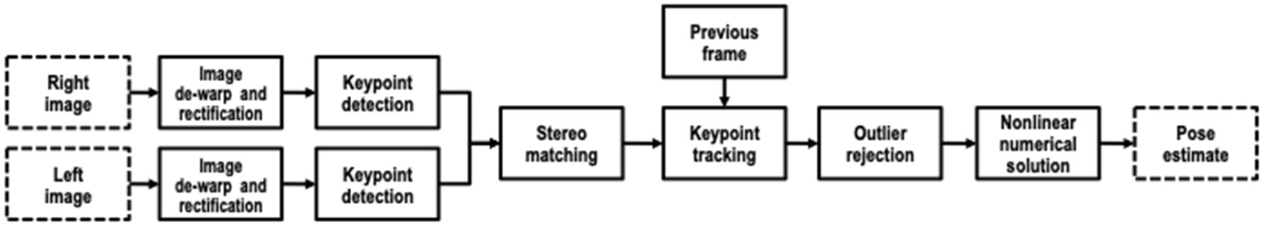
\includegraphics[width=\linewidth]{imgs/stereo_vo.png}
\end{figure}

\textbf{Point Cloud Alignment:} Given \(\bm p_a^j, \bm p_b^j\), minimize cost
\[E(\bm C_{ba}, \bm r_a) = \frac{1}{2}\sum _{j = 1}^J \left(\bm p_b^j - \bm C_{ba}(\bm p_a^j - \bm r_a)\right)^T\bm\Sigma^j\left(\bm p_b^j - \bm C_{ba}(\bm p_a^j - \bm r_a)\right)\]
with matrix weights \(\bm\Sigma^j = \left(\bm G_b^j\bm R_b^j{\bm G_b^j}^T + \bm C_{ba}\bm G_a^j\bm R_a^j{\bm G_a^j}^T\bm C_{ba}^T\right)^{-1}\)
where \(\bm G_b^j = \eval{\pdiff{\bm g}{\bm y}}{\bm f(\bm p_b^j)}, \bm G_a^j = \eval{\pdiff{\bm g}{\bm y}}{\bm f(\bm p_a^j)}\), and $\bm R_b^j, \bm R_a^j$ are pixel measurement covariances.
Closed-form solution for scalar weights:
\begin{enumerate}
	\item Align centroids: $\displaystyle\bm p_a = \frac{\sum _{j = 1}^J w^j\bm p_a^j}{\sum _{j = 1}^J w^j}, \bm p_b = \frac{\sum _{j = 1}^J w^j\bm p_b^j}{\sum _{j = 1}^J w^j}$
	\item Outer product: $\displaystyle\bm W_{ba} = \frac{1}{\sum _{j - 1}^J w^j}\sum _{j = 1}^J w^j(\bm p_b^j - \bm p_b)(\bm p_a^j - \bm p_a)^T$
	\item Compute SVD $\bm V\bm S\bm U^T = \bm W_{ba}$, then compute rotation \(\bm C_{ba} = \bm V\matthree[bsmall]{1}{0}{0}{0}{1}{0}{0}{0}{\det(\bm U)\det(\bm V)}\bm U^T\),
        and translation \(\bm r_a = -\bm C_{ba}^T\bm p_b + \bm p_a\).
\end{enumerate}

Solution is unique if \(\rank\bm W_{ba} \geq 2\). If \(\rank\bm W_{ba} = 2\) points are coplanar (unique if we enforce
no reflection). If \(\rank\bm W_{ba} = 1\) points are colinear.

\subsection{LiDAR Scan Matching}

Given reference $M = \set{\bm p_M^1, \dots, \bm p_M^{N_M}}$, data $D = \set{\bm p_D^1, \dots, \bm p_D^{N_D}}$, where
$N_M = N_D$ (i.e. one-to-one correspondence), find \(\bm T_{MD} = \set{\bm C_{MD}, \bm t_D^{MD}}\).

\textbf{ICP Algorithm:} Until convergence, do:
\begin{enumerate}
	\item Transform $\bm p_M^j = \bm C_k(\bm p_D^j - \bm t_k)$ to form $\tilde D$
  \item Find correspondences $\set{I, J} = \on{NN}(M, \tilde D)$
	\item Error: $\mathcal J = \frac{1}{2}\sum _{j = 1}^J w^j\left(\bm p_M^i - \bm C_k\left(\bm p_D^j - \bm t_k\right)\right)^T\left(\bm p_M^i - \bm C_k\left(\bm p_D^j - \bm t_k\right)\right)$
  \item Gradient descent: $\bm T_{k + 1} = \bm T_k + \alpha\nabla\mathcal J$
\end{enumerate}

\textbf{Subsampling:} \emph{Uniform} (voxel-based): take one point per voxel, preserves structure; \emph{random}:
preserves density, amy lose structure; \emph{feature-based}: identifies structural features to preserve environment
traits; \emph{normal-space}: sample a subset with surface normals uniformly distributed, good for smooth areas with
sparse features.

\textbf{Surface Normal Estimation:} For a neighbourhood of local points, try to fit a plane $a^Tp = c$
by minimizing $\frac{1}{k}\sum _{i = 1}^k (\bm a^T\bm p_i - c)^2$; equivalent to PCA of
$M = \frac{1}{k}\sum _{i = 1}^k (\bm p_i - \bar{\bm p})(\bm p_i - \bar{\bm p})^T$, where the eigenvector of the smallest
eigenvalue (least variance) is the normal.

\textbf{Data Association:} \emph{Closest compatible point}: check normals/colours/etc. within range; \emph{normal
shooting}: first point along the surface normal direction; \emph{outlier rejection} (by checking distances of
neighbours).

\textbf{Point-to-Plane Matching:} Only penalize errors in the normal direction;
\[\mathcal J = \frac{1}{2}\sum _{j = 1}^J w^j\left(\bm p_M^i - \bm C_k\left(\bm p_D^j - \bm t_k\right)\right)^T{\bm n^j}{\bm n^j}^T\left(\bm p_M^i - \bm C_k\left(\bm p_D^j - \bm t_k\right)\right)\]

\textbf{Plane-to-Plane Matching:} Uses normals in both sets;
\begin{tight}
  \[\mathcal J = \frac{1}{2}\sum _{j = 1}^J\left(\bm p_M^i - \bm C_k(\bm p_D^j - \bm t_k)\right)^T(\bm\Sigma _i^M + \bm C_k\bm\Sigma _j^D\bm C_k^T)^{-1}\left(\bm p_M^i - \bm C_k(\bm p_D^j - \bm t_k)\right)\]
\end{tight}

$\bm\Sigma _i^M = \bm C(\bm n_i^M)\bm\Sigma _\varepsilon\bm C(\bm n_i^M)^T$,
$\bm\Sigma _j^D = \bm C(\bm n_j^D)\bm\Sigma _\varepsilon\bm C(\bm n_j^D)^T$,
\(\bm\Sigma _\varepsilon = \diag(\varepsilon, 1, 1)\).

\textbf{Normal Distribution Transform (NDT):} Divide into cells and model each as
$\rho _{c_i}(\bm p) = \exp\left(-\frac{1}{2}(\bm p - \bm\mu _i)^T\bm\Sigma _i^{-1}(\bm p - \bm\mu _i)\right)$;
score each point in \(D\) based on the Gaussian in its cell: $\Lambda(\bm T) = -\sum _{\bm p_D^j \in D}\rho _c(\bm T(\bm p_D^j))$.

\textbf{Practical Considerations:} Motion compensation; anisotropic (e.g. distance-based) filtering to remove
low-information points; coarse-to-fine alignment (starting with smaller subsample); quality estimation via final
association covariance, overlap between scans, etc.

\section{Localization and Mapping} %%%%%%%%%%%%%%%%%%%%%%%%%%%%%%%%%%%%%%%%%%%%%%%%

\textbf{Map Types by Application:} \emph{Planning}: tracks occupancy, safe/unsafe places; \emph{application}: tracks
spatially distributed properties, e.g. topography; \emph{navigation}: tracks localization features, may be sparse.

\textbf{Map Types by Information:} \emph{Metric}: retains scale, metric consistency; \emph{topometric}: locally metric,
globally topographic; \emph{topological}: no distances, just interconnectedness.

\subsection{Occupancy Grid Mapping}

\textbf{Assumptions:} Cell occupancy independent from other cells (no space connectivity) or robot movement,
measurements independent given robot states and map.

\textbf{Probabilistic Update:} \(\displaystyle p(c_k | y^t, x^t) = \frac{p(y_t | c_k, x_t)}{p(y_t)}p(c_k | y^{t - 1}, x^{t - 1})\)

\textbf{Log-Odds:} \(\displaystyle l(x) = \ln\left(\frac{p(x)}{1 - p(x)}\right) \iff p(x) = \frac{\exp(l(x))}{1 + \exp(l(x))}\)

\textbf{Log-Odds Update:} \(\displaystyle l(c_k | y^t, x^t) = l(c_k | y^{t - 1}, x^{t - 1}) + \ln\left(\frac{p(y_t | c_k, x_t)}{1 - p(y_t | c_k, x_t)}\right)\)
where the last term is \(\alpha\) if \(c_k\) near measurement, \(-\beta\) if \(c_k\) closer than measurement, 0 otherwise.

\subsection{Terrain Assessment}

Determine which parts of terrain are safe to traverse and which parts are not by fitting planes to local sections.
Use RANSAC to reject outliers. Use info such as plane height and slope to determine traversibility.

\textbf{Regular Grid}: Patch $j$: let \begin{tight}\(\bm A_j = \matthree{1}{x_{1j}}{y_{1j}}{\newvdots}{\newvdots}{\newvdots}{1}{x_{n_jj}}{y_{n_jj}}, \bm x_j = \cvec{a_j}{b_j}{c_j}, \bm b_j = \cvec{z_{1j}}{\newvdots}{z_{n_jj}}\)\end{tight}
minimize error $\bm e_j = \bm A_j\bm x_j - \bm b_j$, with solution $\bm x_j = (\bm A_j^T\bm A_j)^{-1}\bm A_j^T\bm b_j$.

\textbf{Recursive Formulation:} Let \(\bm p_{ij} = \rvec{1}{x_{ij}}{y_{ij}}{z_{ij}}^T\) and define
\[
\bm P_j = \sum _i \bm p_{ij}\bm p_{ij}^T = \mattwo{\bm A_j^T\bm A_j}{\bm A_j^T\bm b_j}{(\bm A_j^T\bm b_j)^T}{\bm b_j^T\bm b_j}
= \matfour[bsmall]{p_{11}}{p_{12}}{p_{13}}{p_{14}}{p_{21}}{p_{22}}{p_{23}}{p_{24}}{p_{31}}{p_{32}}{p_{33}}{p_{34}}{p_{41}}{p_{42}}{p_{43}}{p_{44}}
= \mattwo{\bm Q^{-1}}{\bm r}{\bm r^T}{p_{44}}
\]
\begin{itemize}
  \item Number of points: $n_j = p_{11}$
  \item Plane fit: \(\rvec{a_j}{b_j}{c_j}^T = \bm Q\bm r\)
  \item Residuals: \(e_j = p_{44} - \bm r^T\bm Q\bm r\)
	\item Average height: $h_j = \frac{p_{14}}{n_j}$
	\item Max slope: $\alpha _j = \cos^{-1}\frac{1}{b_j^2 + c_j^2 + 1}$
\end{itemize}

\subsection{Filtering-Based Localization}

\textbf{Markov Assumption:} The conditional probabilities of future states are independent of any past states, given the
current state; i.e. the state contains enough information to predict the future.

\textbf{Bayes Filter:} \(\displaystyle p(\bm x_k | \check{\bm x}_0, \bm v_{1:k}, \bm y_{0:k}) =\)\\
\(\displaystyle \eta p(\bm y_k | \bm x_k)\int p(\bm x_k | \bm x_{k - 1}, \bm v_k)p(\bm x_{k - 1} | \check{\bm x}_0, \bm v_{1:k - 1}, \bm y_{0:k - 1})\,\dd\bm x_{k - 1}\)

\textbf{Particle Filtering:} Representing the robot state PDF with particles, where each particle is a hypothesis:
\begin{enumerate}
  \item Prediction: $\cvec{\check{\bm x}_{k - 1, m}}{\bm w_{k, m}} \sim p(\bm x_{k - 1} | \check{\bm x}_0, \bm v_{1:k - 1}, \bm y_{0:k - 1})p(\bm w_k)$
        from prior and motion noise; generate predictions \(\check{\bm x}_{k, m} = \bm f(\hat{\bm x}_{k - 1, m}, \bm v_k, \bm w_{k, m})\).
  \item Correction: Assign weights $w_{k, m} = \eta p(\bm y_k | \check{\bm x}_{k, m})$ by using expected measurements
        $\check{\bm y}_{k, m} = \bm g(\check{\bm x}_{k, m}, \bm 0)$ and assuming $p(\bm y_k | \check{\bm x}_{k, m}) = p(\bm y_k | \check{\bm y}_{k, m})$;
        resample based on weights to get new particles \(\hat{\bm x}_{k, m}\).
\end{enumerate}
Practical considerations: Maintaining sample variance by adding more noise, adding samples drawn uniformly from sample
space, or resampling less often; adapting particle count online using weight sum heuristic.

\textbf{Madow Systematic Sampling:} Create $M$ bins where bin $m$ has size $w_{k, m}$; starting from random, take steps
of $1/M$ and sample from each visited bin. Helps preserve particle diversity.

\textbf{Kalman Filter:} Linear model \(\bm x_k = \bm A_{k - 1}\bm x_{k - 1} + \bm v_k + \bm w_k\), \(\bm y_k = \bm C_k\bm x_k + \bm n_k\):
\begin{enumerate}
  \item Prediction: $\twopiece{\check{\bm P}_k = \bm A_{k - 1}\hat{\bm P}_{k - 1}\bm A_{k - 1}^T + \bm Q_k}{\check{\bm x}_k = \bm A_{k - 1}\hat{\bm x}_{k - 1} + \bm v_k}$
  \item Kalman gain: $\bm K_k = \check{\bm P}_k\bm C_k^T(\bm C_k\check{\bm P}_k\bm C_k^T + \bm R_k)^{-1}$
  \item Correction: $\twopiece{\hat{\bm P}_k = (\bm 1 - \bm K_k\bm C_k)\check{\bm P}_k}{\hat{\bm x}_k = \check{\bm x}_k + \bm K_k(\bm y_k - \bm C_k\check{\bm x}_k)}$
\end{enumerate}
With correct modeling KF is \emph{consistent} and \emph{unbiased} (correct mean and covariance).

\textbf{Extended Kalman Filter:} Linearize nonlinear models:
\begin{align*}
  \bm x_k = \bm f(\bm x_{k - 1}, \bm v_k, \bm w_k) &\approx \check{\bm x}_k + \bm F_{k - 1}(\bm x_{k - 1} - \check{\bm x}_{k - 1}) + w_k' \\
  \bm y_k = \bm g(\bm x_k, \bm n_k) &\approx \check{\bm y}_k + \bm G_k(\bm x_k - \check{\bm x}_k) + n_k'
\end{align*}
where \(\bm F_{k - 1} = \pdiff{\bm f}{\bm x_{k - 1}}\), 
\(\bm G_k = \pdiff{\bm g}{\bm x_k}\),
\(\bm w_k' = \pdiff{\bm f}{\bm w_k}\bm w_k\), \(\bm n_k' = \pdiff{\bm g}{\bm n_k}\bm n_k\),
\(\bm f\) Jacobians evaluated at \((\check{\bm x}_{k - 1}, \bm v_k, \bm 0)\) and \(\bm g\) Jacobians at \((\check{\bm x}_k, \bm 0)\).
\begin{enumerate}
  \item Prediction: $\twopiece{\check{\bm P}_k = \bm F_{k - 1}\hat{\bm P}_k\bm F_{k - 1}^T + \bm Q_k'}{\check{\bm x}_k = \bm f(\hat{\bm x}_{k - 1}, \bm v_k, \bm 0)}$
  \item Kalman gain: $\bm K_k = \check{\bm P}_k\bm G_k^T(\bm G_k\check{\bm P}_k\bm G_k^T + \bm R_k')^{-1}$
  \item Correction: $\twopiece{\hat{\bm P}_k = (\bm 1 - \bm K_k\bm G_k)\check{\bm P}_k}{\hat{\bm x}_k = \check{\bm x}_k + \bm K_k(\bm y_k - \bm g(\check{\bm x}_k, \bm 0))}$
\end{enumerate}
where \(\bm Q_k' = \pdiff{\bm f}{\bm w_k}\bm Q_k\left(\pdiff{\bm f}{\bm w_k}\right)^T\),
\(\bm R_k' = \pdiff{\bm g}{\bm n_k}\bm R_k\left(\pdiff{\bm g}{\bm n_k}\right)^T\).
EKF can be biased and inconsistent for severe nonlinearity since it linearizes about the estimate.

\textbf{Sigma Point Transform:} For $L$-dimensional state and parameter \(\kappa\):
\begin{enumerate}
  \item Compute $2L + 1$ sigma points, where \(\bm x_0 = \bm\mu _x\), \(\bm x_i = \bm\mu _x + \sqrt{L + \kappa}\on{col}_i\bm L\),
        and \(\bm x_{i + L} = \bm\mu _x - \sqrt{L + \kappa}\on{col}_i\bm L\), where \(\bm L\bm L^T = \bm\Sigma _x\).
	\item Pass each through the nonlinearity: $\bm y_i = \bm g(\bm x_i)$.
  \item Output Gaussian: \(\displaystyle \bm\mu _y = \sum _{i = 0}^{2L} \alpha _i\bm y_i\),
        \(\displaystyle \bm\Sigma _y = \sum _{i = 0}^{2L} \alpha _i(\bm y_i - \bm\mu _y)(\bm y_i - \bm\mu _y)^T\),
        with weights $\alpha_0 = \frac{\kappa}{L + \kappa}$, $\alpha _i = \frac{1}{2}\frac{1}{L + \kappa}$.
\end{enumerate}

\textbf{Unscented Kalman Filter:}
\begin{tight}
  \begin{enumerate}
    \item State Prediction:
    \begin{enumerate}
      \item Extract sigma points $\bm z_i$ from $\bm\mu _z = \cvec{\hat{\bm x}_{k - 1}}{\bm 0}, \bm\Sigma _{zz} = \mattwo{\hat{\bm P}_{k - 1}}{\bm 0}{\bm 0}{\bm Q_k}$.
      \item Nonlinear motion model: $\bm z_i = \cvec{\hat{\bm x}_{k - 1, i}}{\bm w_{k, i}}$, $\check{\bm x}_{k,i} = \bm f(\hat{\bm x}_{k-1, i}, \bm v_k, \bm w_{k,i})$.
      \item Recombine sigma points: \\
            \(\check{\bm x}_k = \sum _{i = 0}^{2L} \alpha _i\check{\bm x}_{k,i}\),
            \(\check{\bm P}_k = \sum _{i = 0}^{2L} \alpha _i(\check{\bm x}_{k,i} - \check{\bm x}_k)(\check{\bm x}_{k,i} - \check{\bm x}_k)^T\).
    \end{enumerate}
    \item Measurement Prediction:
    \begin{enumerate}
      \item Extract sigma points $\bm z_i$ from $\bm\mu _z = \cvec{\check{\bm x}_k}{\bm 0}, \bm\Sigma _{zz} = \mattwo{\check{\bm P}_k}{\bm 0}{\bm 0}{\bm R_k}$.
      \item Nonlinear measurement model: $\bm z_i = \cvec{\check{\bm x}_{k,i}}{\bm n_{k,i}}$, $\check{\bm y}_{k,i} = \bm g(\check{\bm x}_{k,i}, \bm n_{k, i})$.
      \item Recombine sigma points: $\bm\mu _{y, k} = \sum _{i = 0}^{2L} \alpha _i\check{\bm y}_{k, i}$, \\
            $\bm\Sigma _{yy,k} = \sum _{i = 0}^{2L} \alpha _i(\check{\bm y}_{k, i} - \bm\mu _{y, k})(\check{\bm y}_{k, i} - \bm\mu _{y, k})^T$, \\
            $\bm\Sigma _{xy,k} = \sum _{i = 0}^{2L} \alpha _i(\check{\bm x}_{k, i} - \check{\bm x}_k)(\check{\bm y}_{k, i} - \bm\mu _{y, k})^T$.
    \end{enumerate}
    \item Update: $\bm K_k = \bm\Sigma _{xy,k}\bm\Sigma _{yy,k}^{-1}$, $\twopiece{\hat{\bm P}_k = \check{\bm P}_k - \bm K_k\bm\Sigma _{xy,k}^T}{\hat{\bm x}_k = \check{\bm x}_k + \bm K_k(\bm y_k - \bm\mu _{y,k})}$.
  \end{enumerate}
\end{tight}
UKF deals with nonlinearities better since the approximation is third-order and does not need analytical Jacobians.

\section{Simultaneous Localization and Mapping} %%%%%%%%%%%%%%%%%%%%%%%%%%%%%%%%%%%%%%%%%%%%%%%%

Given frame-to-frame odometric measurements and measurements of landmarks in robot frames, localize the robot and
compute a consistent map of landmarks in the inertial frame.

\subsection{Filtering-Based SLAM}

Filtering-based approaches marginalize out past states, leading to difficulties with large loop closures.

\textbf{EKF-SLAM:} Form augmented state \(\bm x_k\) by stacking robot states and landmark states. Landmarks have
identity motion model with no process noise. Use EKF to estimate robot and landmark positions simultaneously.
Scales poorly with number of landmarks. Can use sparse extended information filter formulation, which sparsifies
\(\bm P^{-1}\) and uses sparsity to quickly invert.

\textbf{Information Filter:} Alternative KF formulation using \(\bm P^{-1}\) and \(\bm P^{-1}\bm x\):
\begin{enumerate}
  \item Prediction: $\twopiece{\check{\bm x}_k = \bm A_{k - 1}\hat{\bm x}_{k - 1} + \bm v_k}{\check{\bm P}_k = \bm Q_k + \bm A_{k - 1}\hat{\bm P}_{k - 1}\bm A_{k - 1}^T}$
  \item Correction: $\twopiece{\hat{\bm P}_k^{-1} = \check{\bm P}_k^{-1} + \bm C_k^T\bm R_k^{-1}\bm C_k}{\hat{\bm P}_k^{-1}\hat{\bm x}_k = \check{\bm P}_k^{-1}\check{\bm x}_k + \bm C_k^T\bm R_k^{-1}\bm y_k}$
\end{enumerate}

\textbf{Rao-Blackwellized Particle Filter/FastSLAM:} Factor the belief as
\(p(\bm x_{1:K}, \bm m | \bm y_{1:K}, \bm u_{1:K}) = p(\bm m | \bm x_{1:K}, \bm y_{1:K})p(\bm x_{1:K} | \bm y_{1:K}, \bm u_{1:K})\),
represent the second piece (robot states) with particle filter, marginalize out first piece (e.g. Gaussians, occupancy
grid). Each particle has its own map; weights are calculated based on measurements and each particle's map.
On loop closure the particles with the most consistent map (best explaining measurements) will remain while others drop out.

\subsection{Batch SLAM}

All poses are kept and globally optimized along with landmark positions, similar to bundle adjustment.
Consider $\bm x_k = \bm f(\bm x_{k - 1}, \bm u_k, \bm w_k)$ and $\bm y_{kl} = \bm g(\bm x_k, \bm m_l, \bm n_k)$, define
errors $\bm e_k = \bm x_k - \bm f(\bm x_{k - 1}, \bm u_k, \bm 0) \sim \mathcal N(\bm 0, \bm Q)$ and 
$\bm e_{kl} = \bm y_{kl} - \bm g(\bm x_k, \bm m_l, \bm 0) \sim \mathcal N(\bm 0, \bm R)$. Minimize error:
\begin{tight}
  \begin{align*}
    J &= \frac{1}{2}\sum _k \bm e_k^T\bm Q^{-1}\bm e_k + \frac{1}{2}\sum _{k,l} \bm e_{kl}^T\bm R^{-1}\bm e_{kl} \\
      &= \alignedlines[t]{}{\frac{1}{2}\sum _k \left(\bar{\bm e}_k + \delta\bm x_k - \bm F_{k - 1}\delta\bm x_{k - 1}\right)^T\bm Q^{-1}\left(\bar{\bm e}_k + \delta\bm x_k - \bm F_{k - 1}\delta\bm x_{k - 1}\right)}{+ \frac{1}{2}\sum _{k, l} \left(\bar{\bm e}_{kl} - \bm G_{x,kl}\delta\bm x_k - \bm G_{m,kl}\delta\bm m_l\right)^T\bm R^{-1}\left(\bar{\bm e}_{kl} - \bm G_{x,kl}\delta\bm x_k - \bm G_{m,kl}\delta\bm m_l\right)} \\
      &= \frac{1}{2}(\bar{\bm e} + \bm E\delta\bm z)^T\bm T^{-1}(\bar{\bm e} + \bm E\delta\bm z)
  \end{align*}
\end{tight}

where \(\bm F = \pdiff{\bm f}{\bm x}, \bm G_x = \pdiff{\bm g}{\bm x}, \bm G_m = \pdiff{\bm g}{\bm m}\), \(\bm T\) has
\(\bm Q, \bm R\) repeated along the diagonal, \(\delta\bm z\) collects perturbations to robot states and landmark
positions, and \(\bar{\bm e}\) collects all odometry and measurement errors.
Solve for optimal update \(\bm E^T\bm T^{-1}\bm E\delta\bm z^* = -\bm E^T\bm T^{-1}\bar{\bm e} \iff \bm A\delta\bm z^* = \bm b\)
and iterate until convergence. \(\bm E^T\bm T^{-1}\bm E\) has a sparse arrowhead structure for fast inversion.

\textbf{Levenberg-Marquardt/Damped Least Squares:} Solve $(\bm E^T\bm T^{-1}\bm E + \mu\diag(\bm E^T\bm T^{-1}\bm
E\delta))\bm z^* = -\bm E^T\bm T^{-1}\bar{\bm e}$ where $\mu$ is tunable and $\diag(\bm A)$ is a matrix with the
diagonal elements of \(\bm A\). Helps when \(\bm A\) is noninvertible and prevents large jumps for highly nonlinear
functions.

\textbf{Line Search:} Search in the direction of $\delta\bm z^*$; do $\bar{\bm z} \gets \bar{\bm z} + \alpha\delta\bm z$
where we pick the largest $\alpha \in [0, 1]$ that decreases $J$.

\textbf{Sliding Window Filter:} Marginalize out old poses and invisible landmarks beyond the sliding window, but keeps
poses within the window; similar to a hybrid of batch and filtering-based SLAM, but still has issues with large loop
closures.

\textbf{Adaptive Relative Bundle Adjustment:} Represent landmark poses relative to observation pose, and robot poses
relative to the last pose to avoid a privileged global frame. Optimize only landmarks and poses within the active
window. Active window size adapts to incorporate more poses and landmarks on loop closure until error is small enough.

\subsection{Visual SLAM}

\subsubsection{Feature-Based SLAM}

Usually consists of a frontend for feature extraction and association (including loop closure), and a backend for map
optimization.

\textbf{MonoSLAM:} First realtime monocular SLAM, using Shi-Tomasi features and constant velocity models. Builds
probabilistic feature map through per-frame bundle adjustment.

\textbf{Parallel Tracking and Mapping (PTAM):} Separate threads for tracking (against existing point cloud) and mapping
(adding to point cloud) into parallel threads. Coarse-to-fine feature matching and local window bundle adjustment for
tracking.

\textbf{Multi-Camera PTAM (MCPTAM):} Extension of PTAM to multiple cameras with non-overlapping FOVs. Spherical
coordinate feature parametrization to limit depth uncertainty to a single axis. Use inverse depth to improve numerical
optimization. Keyframe selection by estimating the amount of covariance reduction in features.

\begin{figure}[h]
  \centering
  \includegraphics[width=\linewidth]{imgs/mcptam.png}
\end{figure}

\textbf{ORB-SLAM:} Improving PTAM with loop closure ORB features. Scale-drift aware loop closure optimizes over and
allows variation of the scale parameter when matching features. Covisbility graph uses viewpoints where features were
observed to filter out implausible features when attempting matching. Bag of Binary Words extracts BoW descriptor from
each frame for relocalization and loop closures. Parallel thread architecture with tracking, local bundle adjustment,
and global loop closure/pose graph optimization, and full bundle adjustment after loop closure. Grid-based ORB feature
extraction to spread out features. Aggressive adding of keyframes, cull when 90\% of points are visible in 3 other
frames.

\textbf{ORB-SLAM2:} Extension of ORB-SLAM for RGB-D input, semi-dense and dense mapping.

\textbf{ORB-SLAM3:} Map atlases for large scale mapping.

\begin{figure}[h]
  \centering
  \includegraphics[width=\linewidth]{imgs/orbslam.png}
\end{figure}

\subsubsection{Direct SLAM}

Match images and produce a pose between frames based on image intensities only, without extracting features, and using
(almost) every pixel to construct the map, i.e. solving pixel correspondence and camera pose estimation at once, instead
of decoupling them like in sparse VO.

\textbf{Comparison to Feature-Based SLAM:}
\begin{enumerate}
  \item More robust to common failure modes due to inclusion of global information, e.g. blur, self-similar textures, defocus
  \item Uses almost all information in the image (as opposed to only pixels around features)
  \item Dense maps enable scene understanding and path planning
  \item Implicit data association by matching pixel intensities
  \item Very high dimensionality ($10^5$ to $10^6$ pixels per image), computationally expensive
  \item Contains a lot more local minima (due to implicit data association), sensitive to initialization (works only for small camera movements); IMU data needed for initialization
  \item No modelling of geometric noise (e.g. rolling shutter)
\end{enumerate}

\textbf{Image Warping:} Given the location of a pixel in frame \(k - 1\) and pose transformation \(\bm T_{k, k - 1}\),
\(\cvec{u_k}{v_k}{d_k} = \bm f\left(\bm T_{k, k - 1}\bm g\left(\cvec{u_{k - 1}}{v_{k - 1}}{d_{k - 1}}\right)\right)\).

\textbf{Photometric Error:} \(e_i = I_{k - 1}(\bm u_{k - 1}^i) - I_k'(\bm u_k^i)\) where \(I_k'\) is interpolated from
\(I_k\), indexed with continuous coordinates \(\bm u_k^i\), and
\(\bm y_k^i = \cvec{\bm u_k^i}{d_k^i} = \bm f(\bm T_{k, k - 1}\bm g(\bm y_{k - 1}^i))\) from image warping.
Solve for optimal pose transform \(\displaystyle \hat{\bm T}_{k, k - 1} = \argmin _{\bm T_{k, k - 1}}\sum _{i = 1}^N\left(\frac{1}{\sigma}e_i\right)^2\).

\textbf{Coarse-to-Fine Optimization:} Starting with a blurred and subsampled image, then repeatedly optimizing while
increasing resolution, using the previous optimization result as the initial guess for the next iteration. First
iteration can use IMU/odometry. This smoothes out local minima and increases region of convergence.

\textbf{Selective Pixel Matching:} Performing matching/optimization only over "informative" pixels, based on gradient
magnitude. Divide image into a grid, and for each cell take only the pixel with the largest gradient magnitude for
optimization.

\textbf{Photometric Calibration:} Dense mapping is affected by gamma, exposure, vignetting, etc., so photometric
calibration can be used to build a model correcting these effects.

\textbf{LSD-SLAM:} Seminal work on direct SLAM.

\begin{figure}[h]
  \centering
  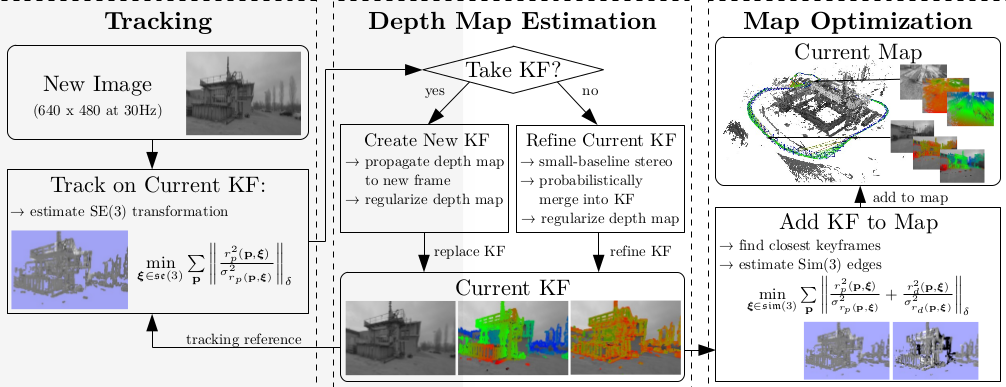
\includegraphics[width=\linewidth]{imgs/lsdslam.png}
\end{figure}

\textbf{Direct Sparse Odometry (DSO):} Integrates photometric calibration and optimizes over a sliding window of 7 keyframes,
fixed number of 2000 active points. Region-adaptive gradient threshold for pixel selection. Try to match pixel along
epipolar line based on motion estimate.

\subsection{LiDAR SLAM}

\textbf{Lidar Odometry and Mapping (LOAM):} Uses a keypoint extractor to look for planes and edges, while avoiding
oblique planes, and edges caused by occlusion; matches only feature points. High-frequency thread performs odometry
and does motion compensation, low frequency thread builds map with fine alignment.

\textbf{Visual LOAM (VLOAM):} Fuses IMU, camera, and LiDAR; high frequency pose propagation using IMU, medium frequency
feature-based visual inertial odometry, then low-frequency corrections from LOAM.

\textbf{LIO-SAM:} Tightly coupled LiDAR-inertial odometry and SLAM, fusing LiDAR along with IMU, GPS, magnetometer, with
a sliding window factor graph for motion correction.

\textbf{LiDAR-Camera-Inertial SLAM Approaches:} \emph{LiDAR-enhanced visual SLAM}: using LiDAR to initialize depths for
bundle adjustment in visual SLAM; \emph{vision-enhanced LiDAR SLAM}: using visual SLAM output poses to initialize scan
registration and pose graph optimization; \emph{tightly coupled}: simultaneous optimization of LiDAR and camera
measurements (BA or BA+PG).

\subsection{Dense RGB-D SLAM}

\textbf{Signed Distance Fields:} Represent surfaces implicitly by storing the signed distance to the nearest surface in
each cell in a voxel grid Max distance often truncated (capped). Recover surfaces from zero crossings using marching
cubes. Noise naturally cancels over time when fusing observations, and surfaces can be represented at sub-voxel
accuracy.

\begin{figure}[h]
  \centering
  \includegraphics[width=0.7\linewidth]{imgs/sdf_confidence.png}
\end{figure}

\textbf{Dense Tracking and Mapping (DTAM):} TSDF fusion from monocular camera. Builds highly detailed maps but requires
many images and suffers with lighting changes and textureless areas. Initialization with feature-based tracking.

\textbf{KinectFusion:} RGB-D dense mapping and odometry using Kinect. Uses TSDF fusion and ICP. Can only map a fixed
volume and relies on slow camera movements.

\textbf{Kintinuous:} Extension of KinectFusion to large-scale maps and adds loop closures. KinectFusion builds small
submaps attached to poses which are loaded dynamically. When loop closure is detected via place recognition, the submap
poses are changed, but their contents are fixed.

\textbf{ElasticFusion:} RGB-D SLAM using surfel maps. Each surfel has a position, normal, radius, colour and confidence.
On loop closure a polygonal mesh is created from the surfel map, elastically deformed, and surfel positions are
recalculated using interpolation.

\textbf{Neural Radiance Field (NeRF) Methods:} Implicit representation of the scene in a neural network. Sacrifices
geometric accuracy but allows rendering realistic views from unseen angles. \textbf{NICE-SLAM} does SLAM using NeRFs in
real time. \textbf{iSDF} uses SDFs stored implicitly in a neural network.

\section{Useful Identities} %%%%%%%%%%%%%%%%%%%%%%%%%%%%%%%%%%%%%%%%%%%%%%%%

\begin{gather*}
  {\textstyle\sin\left(x + \frac{\pi}{2}\right) = \cos(x) \quad \sin\left(x - \frac{\pi}{2}\right) = -\cos(x) \quad \sin\left(\frac{3\pi}{2} - x\right) = -\cos(x)} \\
  {\textstyle\cos\left(x + \frac{\pi}{2}\right) = -\sin(x) \quad \cos\left(x - \frac{\pi}{2}\right) = \sin(x) \quad \cos\left(\frac{3\pi}{2} - x\right) = \sin(x)} \\
  \sin(\bar\theta + \delta\theta) \approx \sin\bar\theta + \cos(\bar\theta)\delta\theta \quad
  \cos(\bar\theta + \delta\theta) \approx \cos\bar\theta - \sin(\bar\theta)\delta\theta \\
  \sin(x + y) = \sin x\cos y + \cos x\sin y \quad \sin(x - y) = \sin x\cos y - \cos x\sin y \\
  \cos(x + y) = \cos x\cos y - \sin x\sin y \quad \cos(x - y) = \cos x\cos y + \sin x\sin y \\
  \sin(\tan^{-1} x) = \frac{x}{\sqrt{1 + x^2}} \qquad \cos(\tan^{-1} x) = \frac{1}{\sqrt{1 + x^2}} \\
  \sin(\cos^{-1} x) = \cos(\sin^{-1} x) = \sqrt{1 - x^2} \\
  \atantwo(-y, x) = -\atantwo(y, x) \qquad \atantwo(y, -x) = \pi - \atantwo(y, x) \\
  \forall a > 0,\,\atantwo(ay, ax) = \atantwo(y, x) \\
  \atantwo\left(x, \sqrt{1 - x^2}\right) = \sin^{-1} x \qquad \atantwo\left(\pm\sqrt{1 - x^2}, x\right) = \pm\cos^{-1} x \\
  \atantwo\left(x, -\sqrt{1 - x^2}\right) = \twocond{\pi - \sin^{-1}x}{x > 0}{-\pi - \sin^{-1}(x)}{x < 0} \\
  v_1 \cdot v_2 = \norm{v_1}\norm{v_2}\cos\theta \qquad v_1 \times v_2 = \norm{v_1}\norm{v_2}\sin(\theta)\hat n \\
  \bm A^{-1} = \frac{1}{\det\bm A}(\on{cof}\bm A)^T \qquad \mattwo{a}{b}{c}{d}^{-1} = \frac{1}{ad - bc}\mattwo{d}{-b}{-c}{a} \\
  \diff{}{x}\sin^{-1}x = \frac{1}{\sqrt{1 - x^2}} \quad \diff{}{x}\cos^{-1}x = -\frac{1}{\sqrt{1 - x^2}} \quad \diff{}{x}\tan^{-1}x = \frac{1}{1 + x^2} \\
\end{gather*}

\textbf{Common Derivatives:} (Denom. layout/gradients are \emph{column vectors})
\begin{gather*}
  \pdiff{}{\bm x} \bm A\bm x = \bm A \qquad \pdiff{}{\bm x} \bm x^T\bm A = \bm A^T \qquad \pdiff{}{\bm x}\bm x^T\bm b = \pdiff{}{\bm x}\bm b^T\bm x = \bm b \\
  \pdiff{}{\bm x}\bm x^T\bm A\bm x = (\bm A + \bm A^T)\bm x \qquad \pdiff{f}{\bm x} = \left(\pdiff{\bm u}{\bm x}\right)^T\pdiff{f}{\bm u} \qquad \pdiff{\norm{\bm x}}{\bm x} = \frac{1}{\norm{\bm x}}\bm x^T \\
\end{gather*}


\end{document}
